\documentclass{article}
\usepackage{graphicx} % Required for inserting images
\usepackage{float}  % Import the float package to use [H] specifier
\usepackage{booktabs}

\setcounter{secnumdepth}{4}

\title{Labwork 4: Threads}
\author{Pham Gia Phuc}
\date{October 2024}

\begin{document}

\maketitle

\setlength\parindent{0pt}

\section{Subject}

    • Copy labwork 3 code to labwork 4 \\
    • Improve labwork 4 code to use 2D blocks \\
    • Use time.time() to measure speedup \\
        
    
\section{Implementation}
    
    This report is using CUDA kernel provided by Google Colaboratory.
    
    \begin{table}[ht]
        \centering
        \begin{tabular}{@{}ll@{}}
            \textbf{Attribute} & \textbf{Value} \\
            Number of CUDA Devices Found & 1 \\
            Device ID & 0 \\
            Name & Tesla T4 \\
            Compute Capability & 7.5 \\
            PCI Device ID & 4 \\
            PCI Bus ID & 0 \\
            UUID & GPU-af936f72-170a-716a-326e-6053e93d8f54 \\
            Watchdog & Disabled \\
            FP32/FP64 Performance Ratio & 32 \\
            Multiprocessor Count & 40 \\
            Approximate Core Count & 2560 \\
            Total Memory Size & 14.75 GB \\
            Environment & Google Colab \\ 
        \end{tabular}
        \caption{CUDA Device Information}
        \label{tab:cuda_device_info}
    \end{table}
    

\section{Results}
    The implementation process utilizes the sample image shown in Figure~\ref{fig:sample-image}.
    

    \begin{figure}[H]
        \centering
        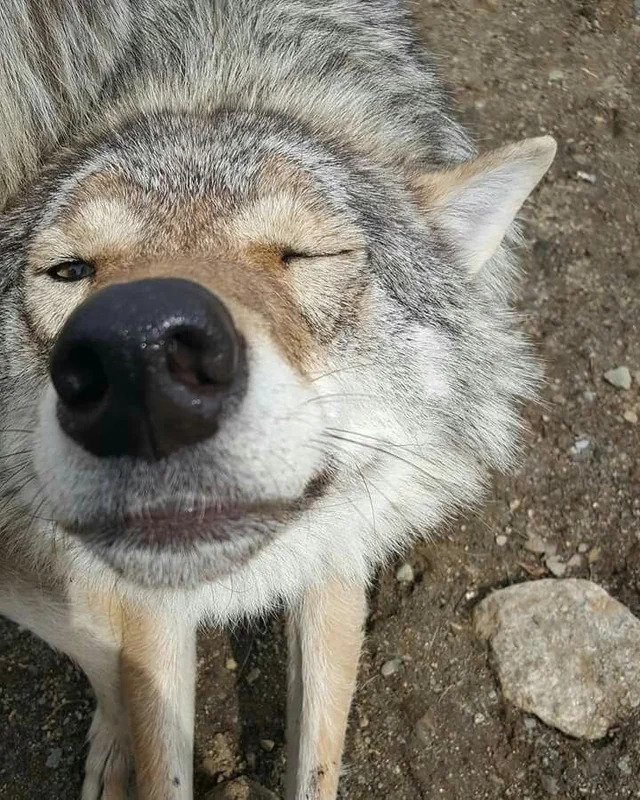
\includegraphics[width=0.5\linewidth]{wolf.jpg}
        \caption{Sample image (Increased resolution)}
        \label{fig:sample-image}
    \end{figure}
    
    \noindent
    The table below shows the information of the image to be processed:
    
    \begin{table}[H]
        \centering
        \begin{tabular}{@{}lll@{}}
            & \textbf{Lab 3} & \textbf{Lab 4} \\
            \textbf{Pixel Count} & 512,000 & 4,995,501 \\ 
        \end{tabular}
        \caption{Image Shape}
        \label{tab:image-shape}
    \end{table}
    
    \noindent
    The table below shows the results of CPU and GPU processing:
    
    \begin{table}[H]
        \centering
        \begin{tabular}{@{}ll@{}}
            \textbf{CPU (seconds)} & \textbf{GPU (seconds)} \\
            0.148201 & 0.005883 \\ 
        \end{tabular}
        \caption{Processing Time}
        \label{tab:processing-time}
    \end{table}

\section{Conclusion}
    The GPU speeds up processing time by 25.19 times compared to the CPU.

\end{document}
